\chapter{The Project}
\label{sec:project}

\cleanchapterquote{TODO.}{TODO}{(TODO)}

%todo
Introduction


\section{Related Works}

%todo knolewdge tree, app: chatboots, study case, Eliza, Alice
knolewdge tree, app: chatboots, study case, Eliza, Alice

\section{The Platforms}

%todo add intro

\subsection{Wit.ai}
%todo fix

\emph{Wit.ai} is \emph{cloud service} that turns speech or text into actionable data.
Wit is supported on every major platform and can be implemented in mobile apps, home automation, wearable devices, robots, and messenger agents.
Thus, it is a interesting \emph{natural language processing} tool for developers.

\subsubsection{History and Background}

\subsubsection{Getting Started}


In this section, we demonstrate the steps to build a voice application on Wit.ai that obtains colour information from voice recognition and changes one html object with it ``on the fly.''
Note that, in order to sign up on Wit.ai and create the voice application, Wit only allow access through a \cite{github_2016} account.

All steps are drawn from \cite{1_wit.ai_2016} Quick Start Guide.
For more details, please refer back to the original source.

%\subsection{The Console}
\emph{The Console}

Once with access to Wit.ai, one is already able to access to what is called the Wit Console. 
The Console is where we can manage the Wit.ai-powered apps, configure a voice app and improve it.
Thus, on the Wit Console App is where the voice applications logic abides.
For instance, the Wit Console with Apps $HelloWorld$ and $ColourTest$ is shown in Figure \ref{fig:console}.
Note that if a user signs in for the first time, Wit.ai creates the first app and the user will land on its page.
We can create new apps from the top-right menu.

\begin{figure}
\label{fig:console}
\centerline{
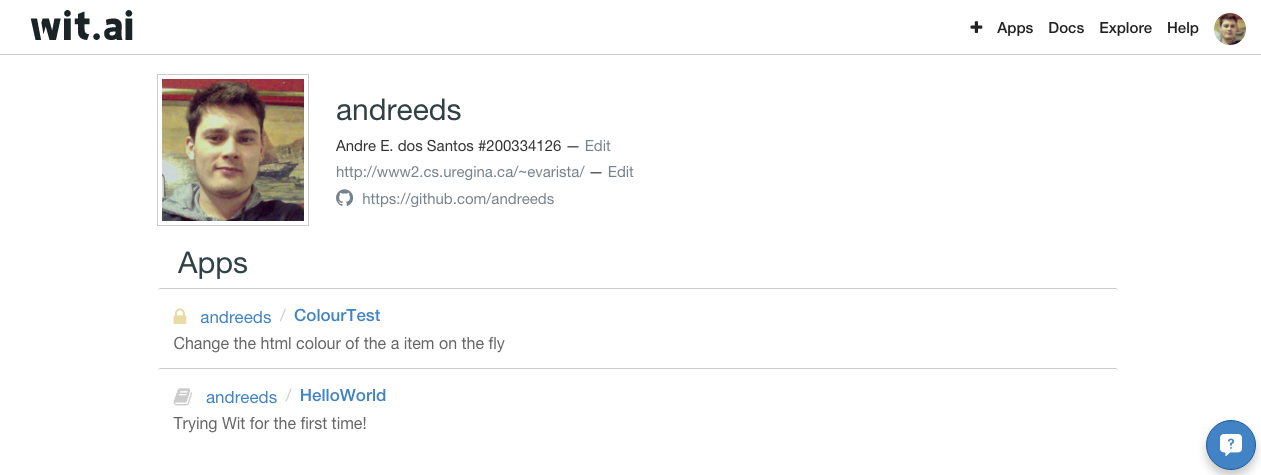
\includegraphics[width=\textwidth]{figures/Wit_Console.png}
}
\caption{The Wit Console.}
\end{figure}

%\subsection{Determining and Creating User Intent}
\emph{Determining and Creating User Intent}

Given that the user has created a new app, it is time to determine the its intents.
An intent is something that the end-user wants to perform.
For example,
``ask about the weather'', 
``set an alarm on their smartwatch'', and 
``say hello to their robot''.
It is common to focus on a finite list of possible intents.
Hence, each intent corresponds to one action in the app.
For our application, the intent is to ``change the colour of the object'' and also``greetings.''

Once with a raw speech or text input, Wit.ai will determine what is the user intent.

For instance, all the following expressions should be mapped to the same intent:
\begin{lstlisting}[language=html]
``Change the colour to blue''
``Colour: blue''
``I want the colour to be blue''
\end{lstlisting}


There are many different ways to express the same intents. 
Thus, it is the job of Wit.ai to map these expressions to actual intents.

The user can browse existing intents from the community of Wit online.
When typing examples for the intents, Wit will suggest these existing intents. 
If one fits the intent, clicking on “GET” gets a copy of the existing intent in the Wit app.
If there not exist an intent that fits, it is necessary to create a new intent.

To create a new intent, the user must type a name for your new intent in the ``Name your intent'' field.
Usually, intent names try to match the app functions or methods. 
At least three expressions, even with synonymous way to say the same command, must be added.
Figure \ref{fig:entents} shows the intents $colour$ and $greeting$ for the ColourTest App.
Some of the expressions for $colour$ are listed in Example \ref{exe:intent}.


\begin{figure*}[!h]
    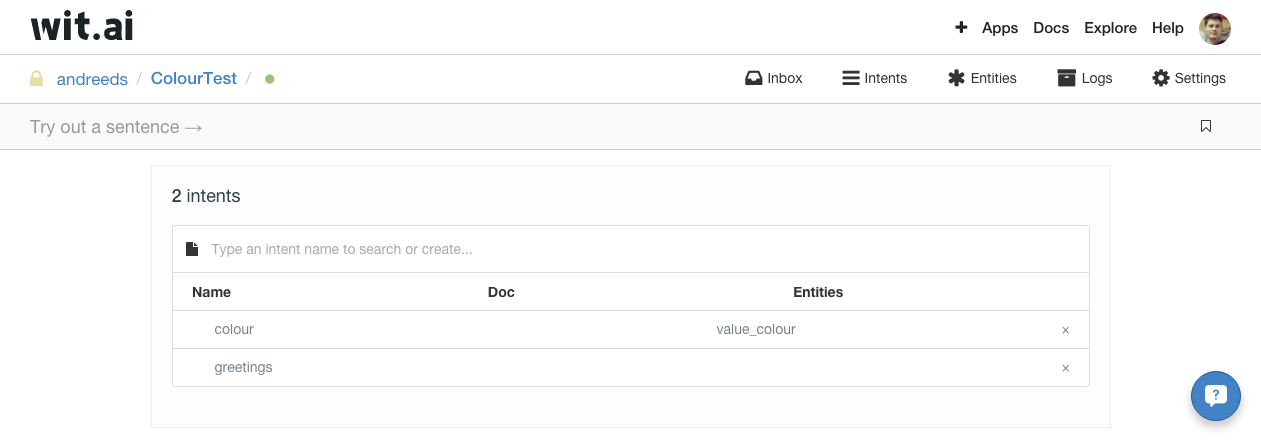
\includegraphics[width=\textwidth]{figures/entities.png}
    \caption{The intents for the ColourTest App.}
    \label{fig:entents}
\end{figure*}


%\subsection{Training}
\emph{Training}

It is time to query the voice app.
At this point, we can already request the voice app via the Wit.ai API.

Notice that, before trainig the app, it is necessary to add the \emph{Client Access Token} to the website.
We will show more details about this step in Section \ref{sec:web}.

In the Inbox of the App we can see the examples said when inputed troght website.

%\subsubsection{Validate Audio from the Inbox}

At Inbox we can validate the the correct sentences recorded by Wit.
Once trained, Wit improves its speech recognitions an the \emph{Confidence} ratio for the expression intents tends to raise.
To train the voice is very simple.
For each expression it reproduces the audio recorded.
If it is correct, we can validate it.
If not, we type the correct sentence and then validate it.

%\subsubsection{Validate Expressions from the Inbox}


At Inbox we can validate matches with expression and intents that were correctly captured by Wit.
For instance, Figure \ref{fig:expressions} shows three expressions captured by Wit, the first one was validated as intent $greetings$, the second was \emph{Archived} since was any of the existing intents, and the third one was validated as intent $colour$.
In our example, we also want to capture the targeted colour.
This is called an \emph{Entity}. 
We can create our own one or select a common one from the dropdown list. 
For instance, the entity $value\_colour$ was created for the intent $colour$, as depicted in Figure \ref{fig:expressions} bottom.


\begin{figure*}[!h]
\begin{center}
    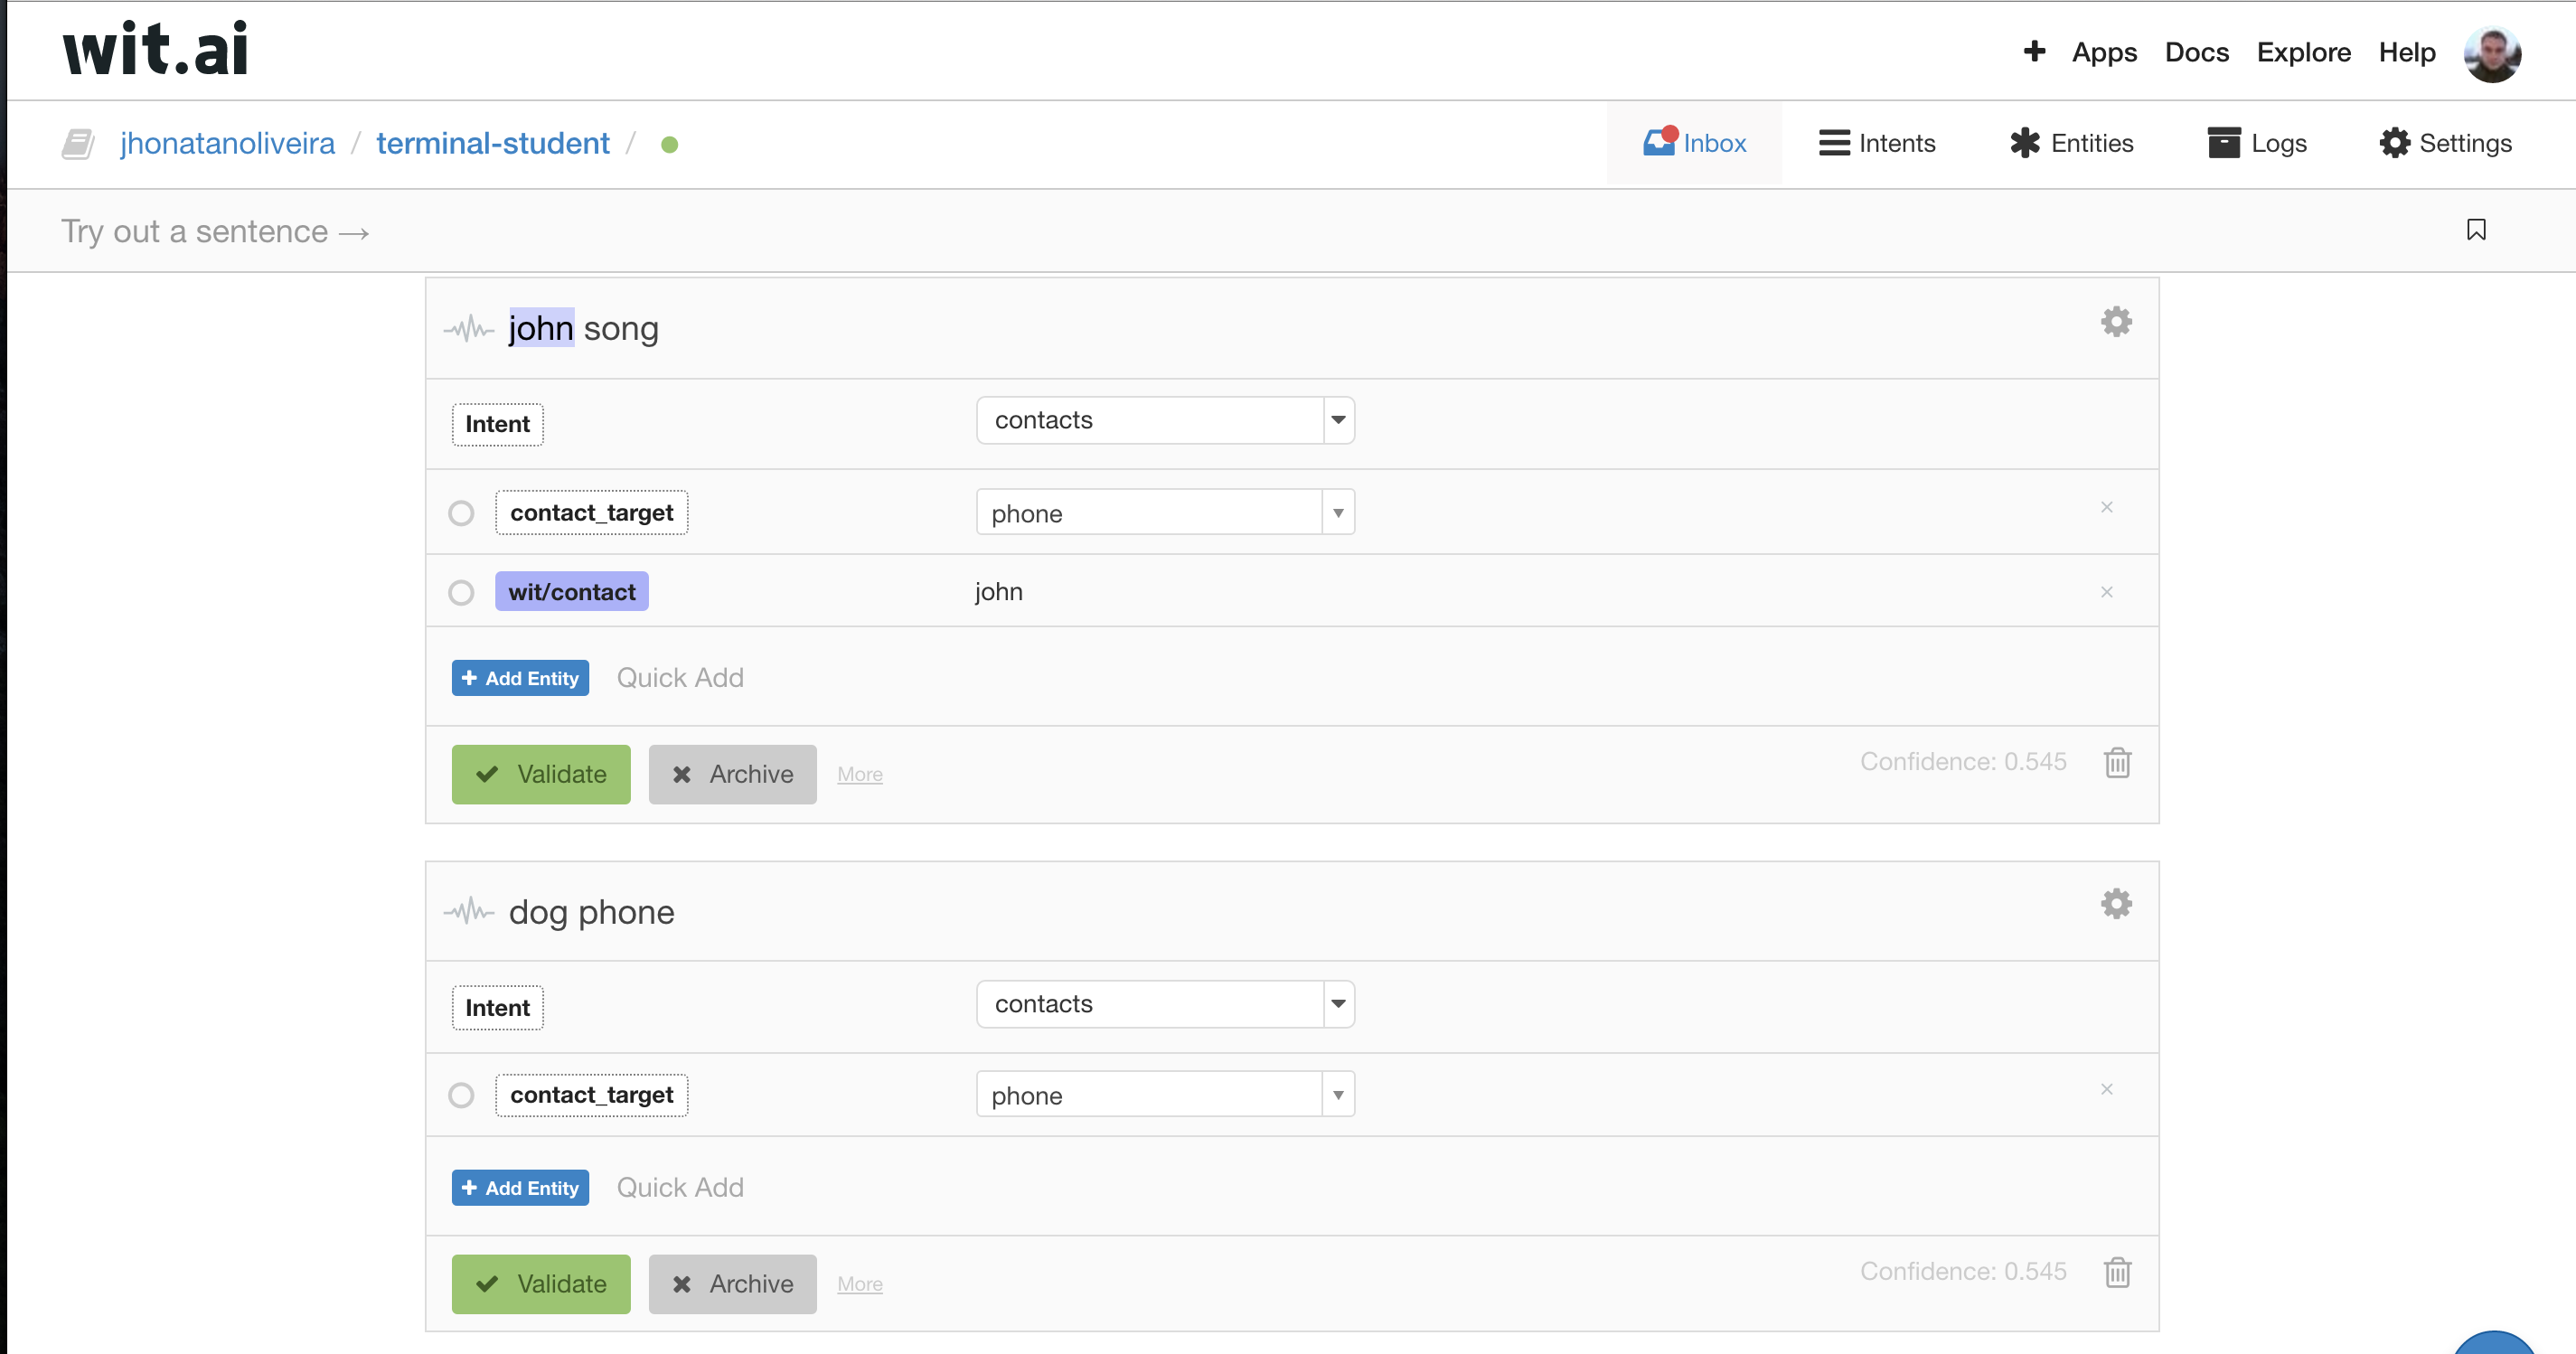
\includegraphics[width=0.75\textwidth]{figures/expressions.png}
    \caption{Expressions captured by Wit.ai.}
    \label{fig:expressions}
\end{center}
\end{figure*}

\subsubsection{Web application}
\label{sec:web}

Now we show how to add Wit to a web app.
As a prerequisites, the browser must support \cite{webrtc}, which is the case of Chrome, Firefox and Opera.

To integrate the voice app with the web app we need to create a new folder for the app, download the \emph{Web SDK} (the microphone app) and extract the archive:
\begin{lstlisting}[language=bash]
	mkdir myapp
	cd myapp
	curl -L <https://github.com/wit-ai/microphone/releases/download/0.7.0/microphone-0.7.0.tar.gz | tar xvzf -
	mv microphone-* microphone
\end{lstlisting}

In the myapp folder, we must create a file $index.html$ containing the html provided by Wit on \url{https://wit.ai/docs/web/0.7.0}.

In the Setting page of the voice app we generate a \emph{Client Access Token}, as illustrated in Figure \ref{fig:token} 
A client access token is unique and authorizes the domain to access the voice app. 
To use the client access token we must replace $CLIENT\_TOKEN$ on the $index.html$ file.
For example, replace 
\begin{lstlisting}[language=java]
	mic.connect("CLIENT_TOKEN");
\end{lstlisting}
for the client access token of our running example, given
\begin{lstlisting}[language=java]
	mic.connect("AWRBY6WLIPAQP7PGCGMQQKKO45LELCWO");
\end{lstlisting}

\begin{figure*}[!h]
\begin{center}
    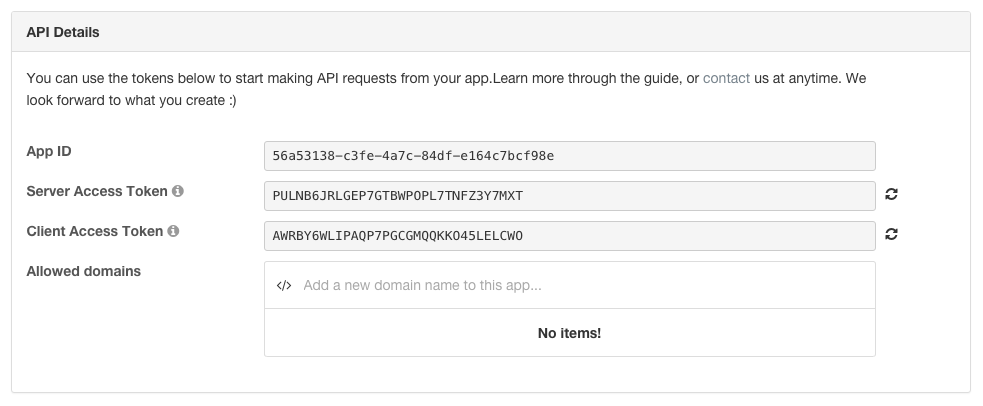
\includegraphics[width=0.75\textwidth]{figures/token.png}
    \caption{A Client Access Token.}
    \label{fig:token}
\end{center}
\end{figure*}


%\subsection{In Action}
\emph{In Action}

To see the web application in action we serve the app with a webserver.
For instance, using Python:
\begin{lstlisting}[language=bash]
	python -m SimpleHTTPServer
\end{lstlisting}
Then, to load the page on the browser
\begin{lstlisting}[language=bash]
	http://localhost:8000
\end{lstlisting}



After allowing your microphone, we will be able to click on the microphone icon and say a command. 
The command will be streamed to the voice app.


\subsubsection{Resource Constrains}



\subsection{Meteor.js}

\emph{Meteor.js} \cite{meteor}, or Meteor for short, is an open-source web platform to create applications using the Web 2.0 paradigmas.
The platform provide a reactive approach by focusing on the data flow.
This is done by creating and managing events in the application.
Also, data management is done with a non-SQL database called \emph{MongoDB} \cite{mongo}.
Meteor simplify the application development by providing an unique programming language, javascript, throughout the whole stack process.
Moreover, the platform makes available a set of common tools for business logic and data management.
Finally, Meteor deploys the application in desktop and mobile without needing to change the source code.

\subsubsection{History and Background}

The Meteor platform was created by a company called Skybreak in 2011 \cite{skybreak}.
Later, in 2012, the company changed its name to Meteor.
The startup was incubated by YCombinator \cite{ycomb} and after receiving an investment of \$11.2 M, the platform development increased considerably.
The platform left beta in October 26th, 2015, with a version that currently provides multiplatform support.

Regarding its internal structure, Meteor is built on top of \emph{Node.js} \cite{node}.
That means that Meteor is driven by events, in order to create an asynchronous model.
This feature is implemented using callback functions: when an event happens a specific function is called to execute a portion of code.
The server-side and client-side are both implemented using javascript.
In the client-side, templates are used to design user interfaces.
Here, a simple markup language defines the design and the events handled by the application.
Meteor has support for more than one template language, being \emph{Blaze} \cite{meteor} the official one.
In the server-side, Meteor handles data management using collections.
The oficial non-SQL database supported is MongoDB, but new ones are being incorporated in future versions \cite{fathom}.


\subsubsection{Getting Started}

Now, we will follow a common flow for an app creation process.
During this section, we will use a single running example which is an application for todo lists.
This todo example can also be found on the official getting started tutorial in \cite{meteor}.
We will try to keep the same code conventions and names always that possible so the reader can use this paper as an extended guide for that tutorial.
We assume that the Meteor program and required 

The following command line is used to create a new application with Meteor:
\begin{lstlisting}[language=bash]
meteor create todo
\end{lstlisting}
This creates a folder structure as shown below:
\begin{lstlisting}[language=bash]
todo.js todo.html todo.css .meteor
\end{lstlisting}
The \emph{todo.js} file is where the javascript code for the server and client stays.
Here is where the code throws and handles events, besides business logic.
Templates for user interface is done in the \emph{todo.html} file with pure HTML markup language and a template markup language.
For this project Blaze is the template languages used.
The \emph{todo.css} file contains styles for the templates.
Lastly, the \emph{.meteor} stores settings and the meteor aplication itself in a hidden folder.

%\subsubsubsection{Templates}
\emph{Templates}

Templates are defined using a special tag called \emph{template}.
Once defined, a template can be included within any HTML code.
In this way, a template is a interface module that can be reuses wherever it is required.
All the HTML code and the templates have access to the data made available in that part of the HTML code.
The basic flow is: the javascript code makes available some data to a specific area of the HTML code (or a specific template), so the template language can access that data and print the ones of interest for the user.
Bellow, we show a simple todo list interface.

\begin{lstlisting}[language=html,escapechar=|]
<head>
  <title>Todo List</title>
</head>
 
<body>
  <div class="container">
    <header>
      <h1>Todo List</h1>
      <form class="new-task">  |\label{code:form_b}|
        <input type="text" name="text" placeholder="Type to add new tasks" />
      </form>  |\label{code:form_e}|
    </header>
 
    <ul>
      {{#each tasks}}
        {{> task}} |\label{code:temp}|
      {{/each}}
    </ul>
  </div>
</body>
 
<template name="task">  |\label{code:temp_b}|
  <li class="{{#if checked}}checked{{/if}}"> |\label{code:checked}|
    <button class="delete">&times;</button>  |\label{code:delete}|
    <input type="checkbox" checked="{{checked}}" class="toggle-checked" />
    <span class="text">{{text}}</span>
  </li>
</template>  |\label{code:temp_e}|
\end{lstlisting}

Here, the HTML code defines in its \emph{body} a title and a list.
Notice that Blaze commands are defined within \emph{\{\{} and \emph{\}\}}.
In the list, the Blaze command \emph{\#each} goes through a list of data, as in a loop lace.
The data variable \emph{tasks} contains this list of data and was made available to this part of the code by the javascript code.
The Blaze command \emph{$>$ name\_of\_template} prints a template previously defined with name \emph{name\_of\_template}.
In lines \ref{code:temp_b}-\ref{code:temp_e}, the template named \emph{task} is defined.
This template expect to find available in its scope a data variable called \emph{text}.
In line \ref{code:temp}, the template is included in that spot of the HTML code and the data variable \emph{text} is available on the loop scope of the \emph{\#each} command.
Note that \emph{text} is a field within \emph{tasks}.

On the javascript file we define code for the client and server.
In order to distinguish between them, Meteors makes available a global variable called \emph{isClient}, which goes to true if the running environment is the browser and goes to false if it is the Node.js one.
If a code is called without being under the conditions of a client or server, the code is run in both environments.
Follows the javascript code to create a simple database where the \emph{tasks} are saved.

\begin{lstlisting}[language=java,escapechar=|]
Tasks = new Mongo.Collection("tasks");  |\label{code:db}|
 
if (Meteor.isClient) {  |\label{code:cond}|

  // This code only runs on the client
  Template.body.helpers({  |\label{code:help_b}|
    tasks: function () {  |\label{code:func}|
      return Tasks.find({});
    }  |\label{code:help_e}|
  });
  
  Template.body.events({
    "submit .new-task": function (event) {  |\label{code:event}|
      // Prevent default browser form submit
      event.preventDefault();
 
      // Get value from form element
      var text = event.target.text.value;
 
      // Insert a task into the collection
      Tasks.insert({
        text: text,
        createdAt: new Date() // current time
      });
 
      // Clear form
      event.target.text.value = "";
    }
  });
  
  Template.task.events({
    "click .toggle-checked": function () {  |\label{code:event_checked}|
      // Set the checked property to the opposite of its current value
      Tasks.update(this._id, {
        $set: {checked: ! this.checked}
      });
    },
    "click .delete": function () {  |\label{code:delete_java}|
      Tasks.remove(this._id);
    }
  });
  
}
\end{lstlisting}

Line \ref{code:db} runs on the server and on the client, since it is not inside the conditional in line \ref{code:cond}.
In the server, that command creates a database called \emph{tasks} if it does not exist already.
In the client, it creates a cache of the same database where Meteor manages some saved data in order to reuse repeated queries from the user.
From line \ref{code:help_b} to \ref{code:help_e}, using the global variable \emph{Template}, we make available to the \emph{body} of the HTML whatever data the not named function in line \ref{code:func} return.
The function returns all the entries in the previously created \emph{tasks} database.
These returned data is available to the HTML code on a data variable called \emph{tasks}, as determined in line \ref{code:func}.

%\subsubsubsection{Inserting Data}
\emph{Inserting Data}

Regarding the data inclusion, this HTML code has a form which will receive the new input data from the user.
Lines \ref{code:form_b}-\ref{code:form_e} defines a simple form where the user can input new tasks.
When pressing enter, an event is thrown from the HTML code and can be handled in the javascript code.

The javascript code watch for an event for the form submission, as shown in line \ref{code:event}.
From here, the default reaction of the browser, which is try to submit the form, is stopped.
The, the value of the input text is saved in a variable.
Next, the cached database variable \emph{Tasks} is used to insert a new entry on the server database with the text saved from the user input.
Finally, the text input is cleared.

Notice in the last insertion process that the cached database was used to update the server database.
This is possible due to the way Meteor works in client and server.
The client has only a cached version of the database.
But whenever this cached version is updated, an event goes to the server (whenever there is connection available) making the server database to update.
The other way around works in the same manner: if the server database is updated, an event goes to all client spreading the update.

%\subsubsubsection{Updating and Removing Data}
\emph{Updating and Removing Data}

If a task is done, we want to check it out from the list by updating its entry with a done flag.
In the HTML code, line \ref{code:checked}, the template \emph{task} has a conditional statement checking for a variable called \emph{checked}.
If the variable is true, the body of the condition, which is just a string \emph{checked}, is executed.
This variable, as expected, is set in the javascript code.
Indeed, in line \ref{code:event_checked}, the javascript watch for an event of a click on the checkbox.
If it happens, the cached database \emph{Tasks} is updated by setting a field \emph{checked} to the opposite value that the user entered.
Notice the use of a special variable \emph{this} which provides context for HTML access from where the event occurred.


The deletion process is similar to updating but a different function is used on the cached database.
The javascript code, line \ref{code:delete}, watch for the HTML code, line \ref{code:delete}.
When the user clicks in the delete button, the javascript code is executed by removing the correspondent id of the entry.
Again, note the use of \emph{this} as a context variable for the entry where the event occurred.

\subsubsection{Resource Constrains}

Meteor can be used to build resource constrain products.
In this type of application, the amount of processing and memory are often restricted.
Therefore, the use of parallel computing or decentralized tasks are common and necessary.
Meteor can be use to avoid heavy load computation in the limited hardware itself.
A server can be used to process all the required heavy workload while the client simply show in real time the results.

One way of providing an interface to a Meteor server side is by using the official server-client protocol, called \emph{Distributed Data Protocol} (DDP).
The DDP protocol is a simple specification on how other languages can communicate with a Meteor server.


\subsection{Raspberry Pi}

%todo add photo resppi
The \emph{Raspberry Pi} a low cost is single-board computer developed in the UK by the Raspberry Pi Foundation with the intention of stimulating the teaching of basic computer science in schools \cite{pi2012raspberry}.
It is a capable small device that is capable of doing everything a desktop computer does, from browsing the internet and playing high-definition video, to making spreadsheets, word-processing, and playing games \cite{resp2}.

The Raspberry Pi has a Broadcom BCM2835 system on a chip (SoC), which includes an ARM1176JZF-S 700 MHz processor, VideoCore IV GPU, and 256 megabytes of RAM. 
It uses an SD card for booting and long-term storage.
The Raspberry Pi 2 Model B is the second generation Raspberry Pi. 
It replaced the original Raspberry Pi 1 Model B+ in February 2015. 
Compared to the Raspberry Pi 1 it has: (i) A 900MHz quad-core ARM Cortex-A7 CPU and (ii) 1GB RAM \cite{resp2}.



\subsubsection{History and Background}

%todo adjust
In 2006, early concepts of the Raspberry Pi were based on the Atmel ATmega644 microcontroller \cite{wong2011build}.
The Model A was not the first Raspberry Pi to hit general availability – that distinction went to the Model B. 
The A was, nevertheless, the truest to the bare-bones ethos of the Pi project, retailing for \$25 and initially packing just 128MB of memory. (Later raised to 256MB.)

\subsubsection{Getting Started}

Required:
SD Card. The newer Raspberry Pi Model A+, Raspberry Pi Model B+, Raspberry Pi 2 Model B, Raspberry Pi Zero, and Raspberry Pi 3 Model B require micro SD cards.
Display and connectivity cables
Keyboard and mouse
Power supply

Not essential but helpful to have

    Internet connection
        To update or download software, we recommend that you connect your Raspberry Pi to the internet, either via an Ethernet cable or a WiFi adapter.


Plugging in your Raspberry Pi

Before you plug anything into your Raspberry Pi, make sure that you have all the equipment listed above to hand. Then follow these instructions:

    Begin by slotting your SD card into the SD card slot on the Raspberry Pi, which will only fit one way.
    Next, plug your USB keyboard and mouse into the USB slots on the Raspberry Pi.
    Make sure that your monitor or TV is turned on, and that you have selected the right input (e.g. HDMI 1, DVI, etc.).
    Then connect your HDMI cable from your Raspberry Pi to your monitor or TV.
    If you intend to connect your Raspberry Pi to the internet, plug an Ethernet cable into the Ethernet port next to the USB ports, otherwise skip this step.
    When you are happy that you have plugged in all the required cables and SD card, plug in the micro USB power supply. This action will turn on and boot your Raspberry Pi.
    If this is the first time your Raspberry Pi and NOOBS SD card have been used, then you will have to select an operating system and configure it. Follow the NOOBS guide to do this.

Read more in our documentation.

\subsubsection{Resource Constrains}

The main disadvantages of Raspberry Pi are \cite{vujovic2014raspberry}:

It does not have a real-time clock (RTC) with a backup battery but it can easily work around the missing clock using a network time server, and most operating systems do this automatically.

It does not have a Basic Input Output System (BIOS) so it always boots from an SD card.

It does not support Bluetooth or WiFi out of the box but these supports can be added by USB dongles.

Unfortunately, most Linux distributions are still a bit
picky about their hardware, so it should be first checked whether flavor of Linux supports particular device.

It doesn’t have builtin an Analog to Digital converter. External component must be used for AD conversion.

It has a relatively small number of digital I/O, but it can be expanded with external logic devices.

\section{Implementation}

%- Administration scheme:
%    - Services
%        - Data
%            - Knowledge tree
%                - The tree is built in server not in client
%        - External
%            - Map with key-value being the key the name of the external service and the value a function which runs the service
%- Searching the tree
%    - scoring the tree with one pass
%    - problem: when we have the query found in the parent and child. Eg: tainara -> tainara@gmail.com


How the project works.

- Administration scheme:
    - Services
        - Data
            - Knowledge tree
                - The tree is built in server not in client
        - External
            - Map with key-value being the key the name of the external service and the value a function which runs the service

- Searching the tree
    - scoring the tree with one pass
    - problem: when we have the query found in the parent and child. Eg: tainara -> tainara@gmail.com

% add as section:  Description of design process
\subsection{Description of design process}

The design process of our project is based on three different platforms, including two cloud computing ones, namely Wit.ai and Meteor.js, and one hardware, Raspberry Pi.
The overview design is a system implemented in Meteor.js containing a server and a client.
Here, the server is a more powerful computer, capable of processing exhaustive algorithms.
Thus, the server is used as a central processing unit and only forward responses for the client's processing requests.
The client is considered a less powerful computer, which receives orders from the user and send processing requests to the server.
This design process is managed by Meteor.js by using its clear division between client and server code.

The main idea in this division is to allow the client to make calls to functions implemented inside the server.
These functions, in the other hand, returns plain text in json format to the client.
In this way, a client would require only processing power enough to make the request.
Our project focus on the Raspberry Pi.
Then, whenever a processing algorithm requires too much power, we transfer that to the server side of the code.

The requests from the user is treated by the Wit.ai platform.
We use its natural language processing capabilities to understand the user's query and send the proper request to the server.
This processing is done in a search within a knowledge tree, also saved on the server.

%add as section:Discussion of group contributions
\subsection{Discussion of group contributions}



\section{Results}

The system was implemented successfully with only one change in the original idea, which is not crucial to this demonstration.
Our focus with the project was to use clouding platforms to overcome hardware platform limitations.
In this way, we could make a system that interact with the user by a terminal client using a Raspberry Pi, and replies to the user by processing the query on the server side.
The only feature we could not implement was the indoor navigation capability.
This failure in our plans is further described in Section \ref{sec:ex-project}, as we also discuss the context and alternatives that we tried in more detail.
Now, we describe and show our implemented system.

The administrator log in the system using its unique account.
For now, this is fixed and set automatically by the system on startup.
For test purposes, the current username is \emph{admin} and password \emph{cs8072016}.
The welcome page, shown in Figure \ref{fig:sys_welcome}, means a successful log in.
This page has no useful information, but it was created thinking in a possible dashboard with overview statistics of the whole system.

\begin{figure}[htbp]
\begin{center}
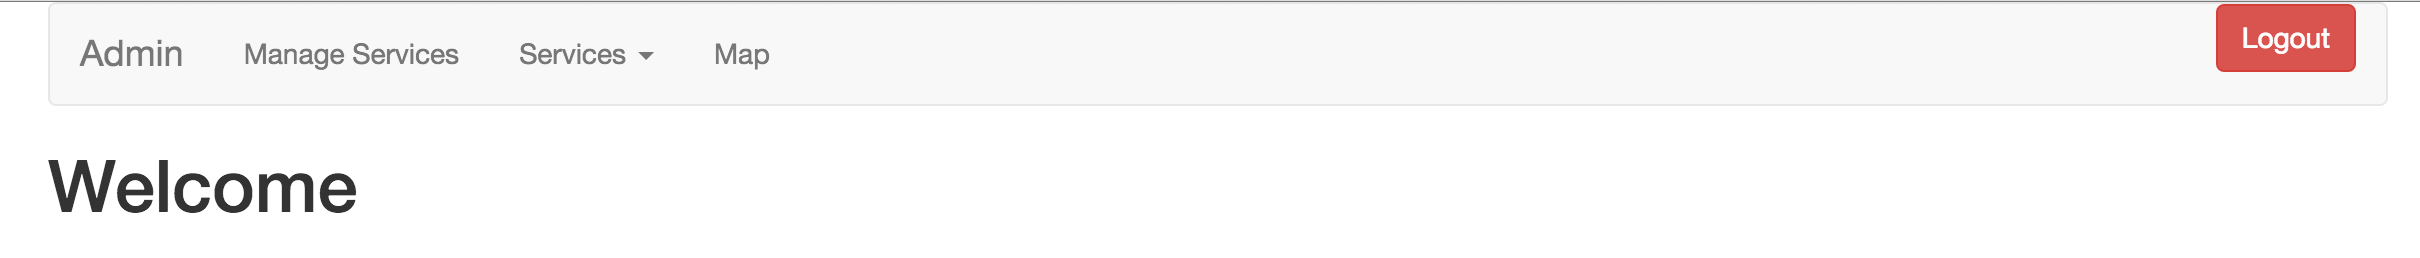
\includegraphics[width=\textwidth]{figures/welcome.png}
\caption{Welcome page at the administrative side of the system. Future work might include a dashboard at this page.}
\label{fig:sys_welcome}
\end{center}
\end{figure}

Adding services to the system can be done by using the top menu bar.
In ``Manage Services'', depicted in Figure \ref{fig:sys_mang_serv}, the administrator can create and delete services that are available for the user.
These services are of two types: data services and external services.
The data service is internally described by a knowledge tree.
All corresponding knowledge trees can be edited in this same administrator screen (as described next).
The external service is configured in a hash map in code.
This is a flexible way of adding external APIs within the system.
Whenever the administrator wants to make an API available to the user, one more pair of ``key-value'' needs to be added to that hash map.
Figure \ref{fig:sys_add_serv} shows a popup used to add both type of services.

\begin{figure}[htbp]
\begin{center}
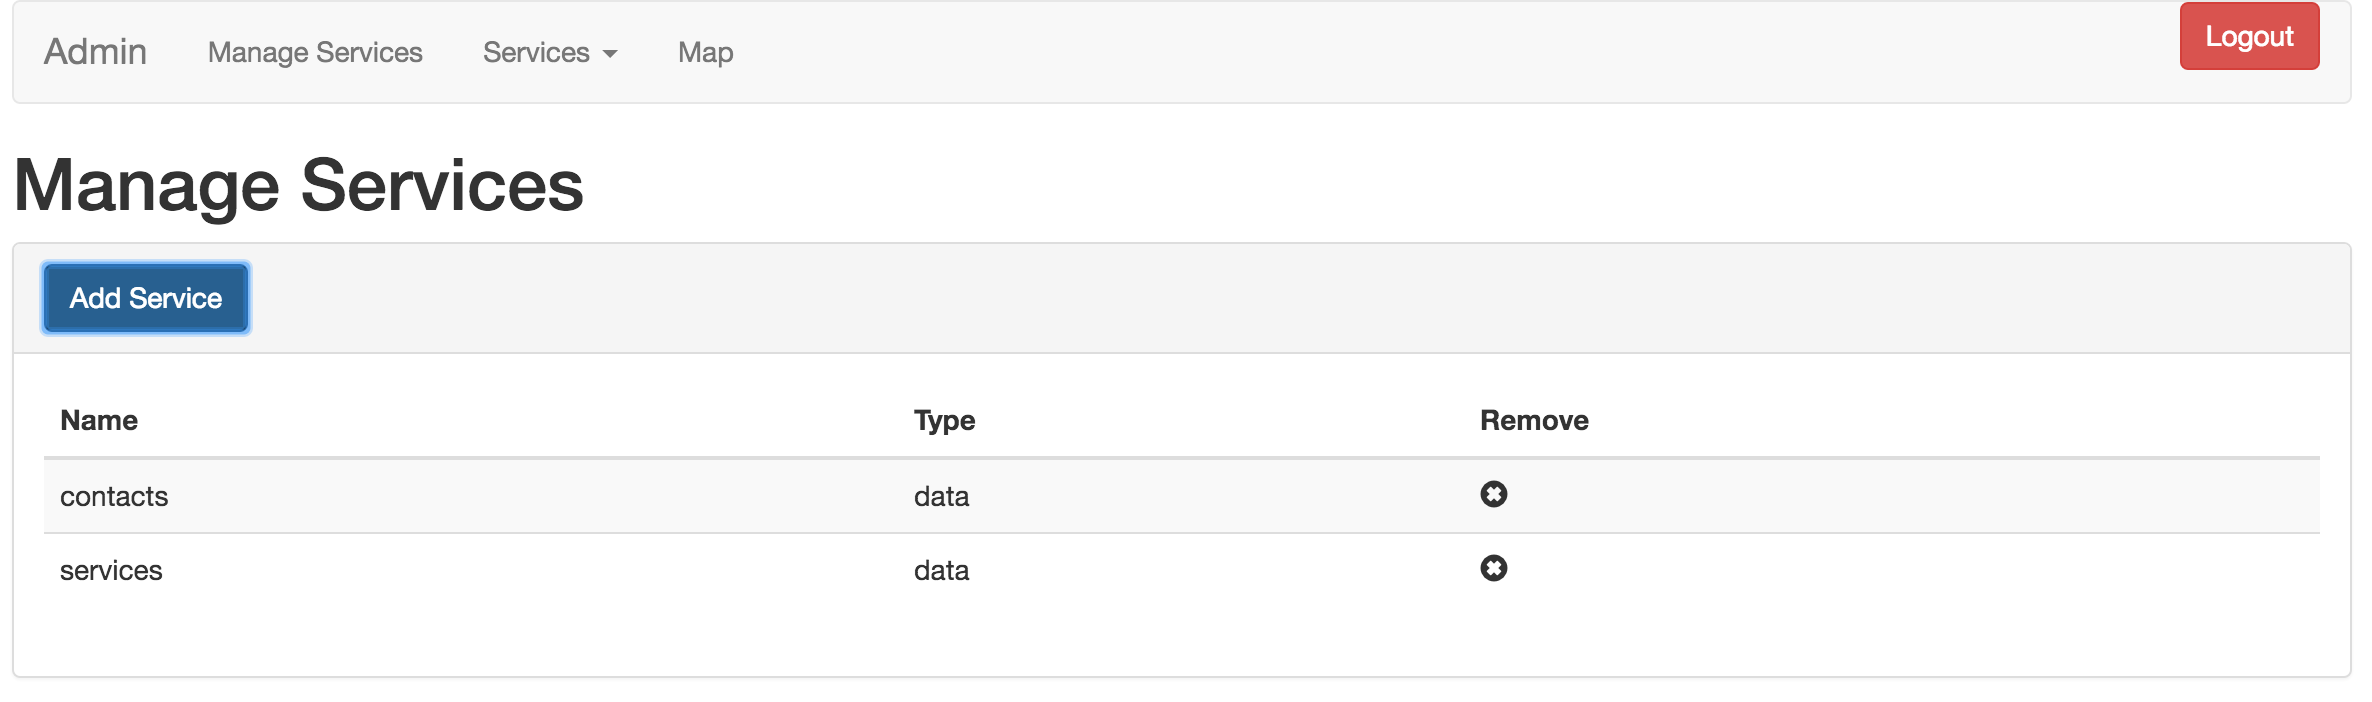
\includegraphics[width=\textwidth]{figures/manage_serv.png}
\caption{Add and remove services within the System. There are available two types of services: data and external. The former is described by a knowledge tree, while the later is described by an external API.}
\label{fig:sys_mang_serv}
\end{center}
\end{figure}

\begin{figure}[htbp]
\begin{center}
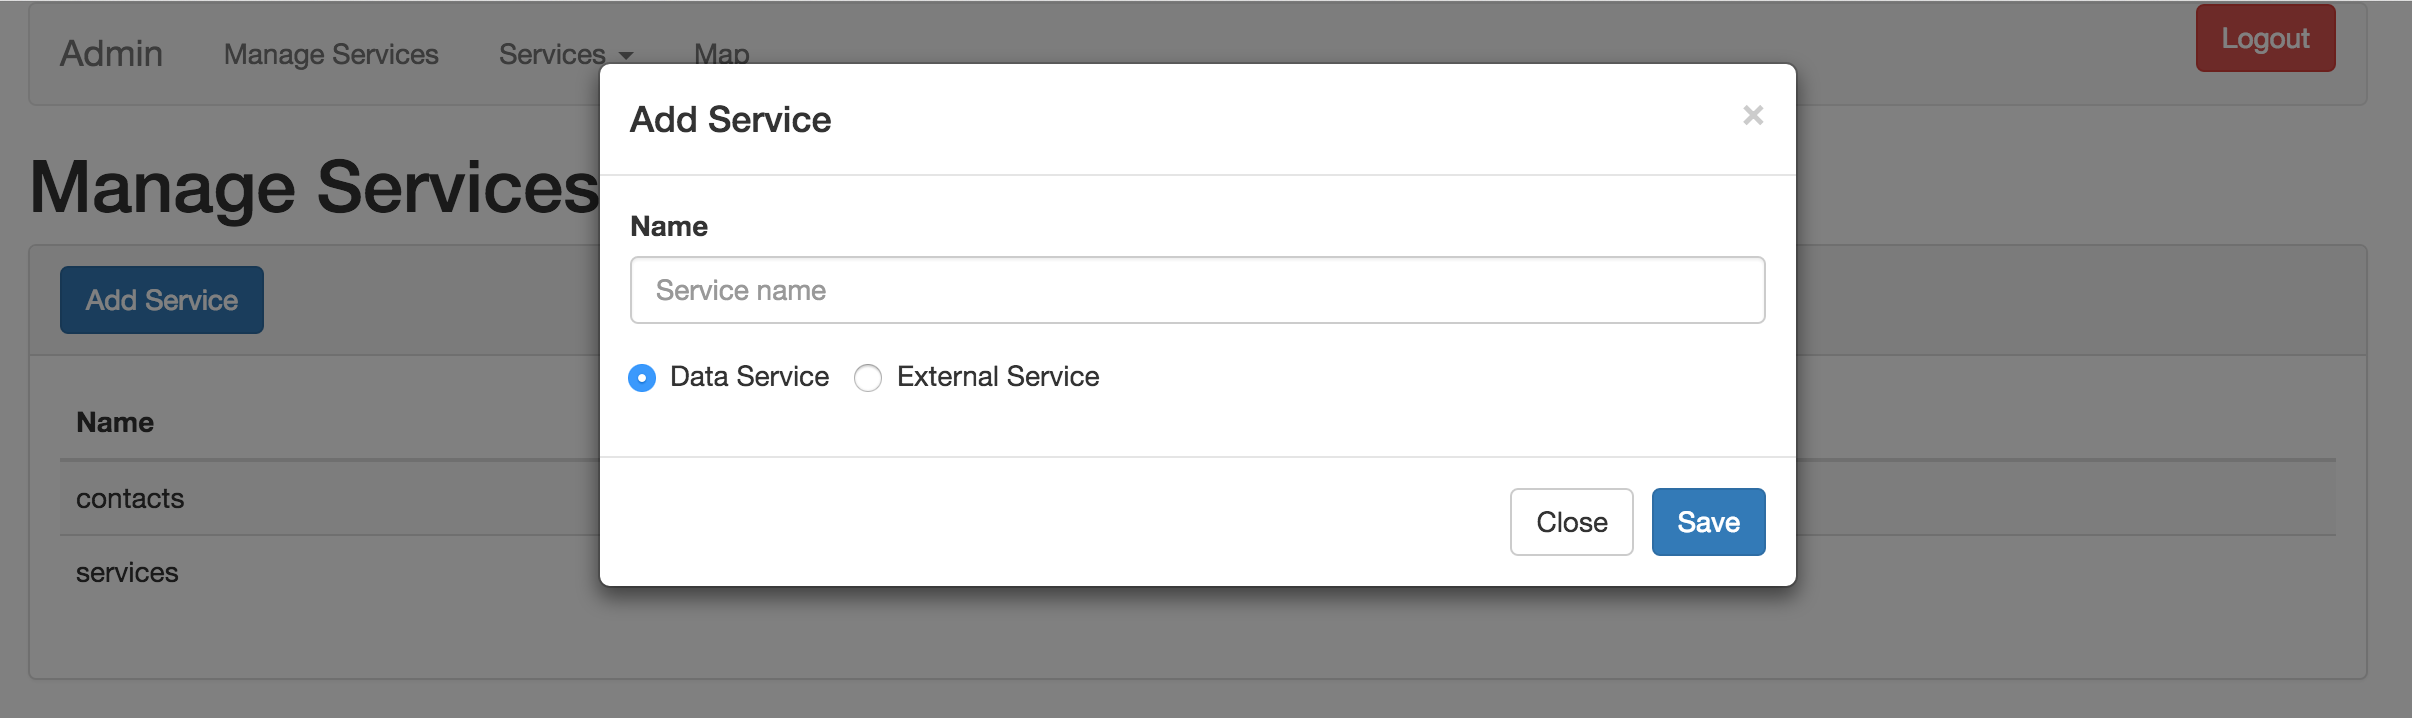
\includegraphics[width=\textwidth]{figures/add_serv.png}
\caption{Popup to add a new service.}
\label{fig:sys_add_serv}
\end{center}
\end{figure}

Now, the data service type can be fully edited inside this administrator screen.
As illustrated in Figure \ref{fig:sys_serv}, the administrator has a visual tool to expand/contract the branches of the tree.
Using the tools in the right hand side, nodes can be added, removed and its label edited.
Notice that removing a node also removes all its descendants.
A sandbox for testing user queries is also added within this screen.
In this way, the user can test a query on the fly, just like the user would ask.
The answer is then depicted in the knowledge tree in the left hand side.
Since this knowledge tree can always be edited, these available tools can be powerful for modelling a whole problem domain and testing them at the same time.

\begin{figure}[htbp]
\begin{center}
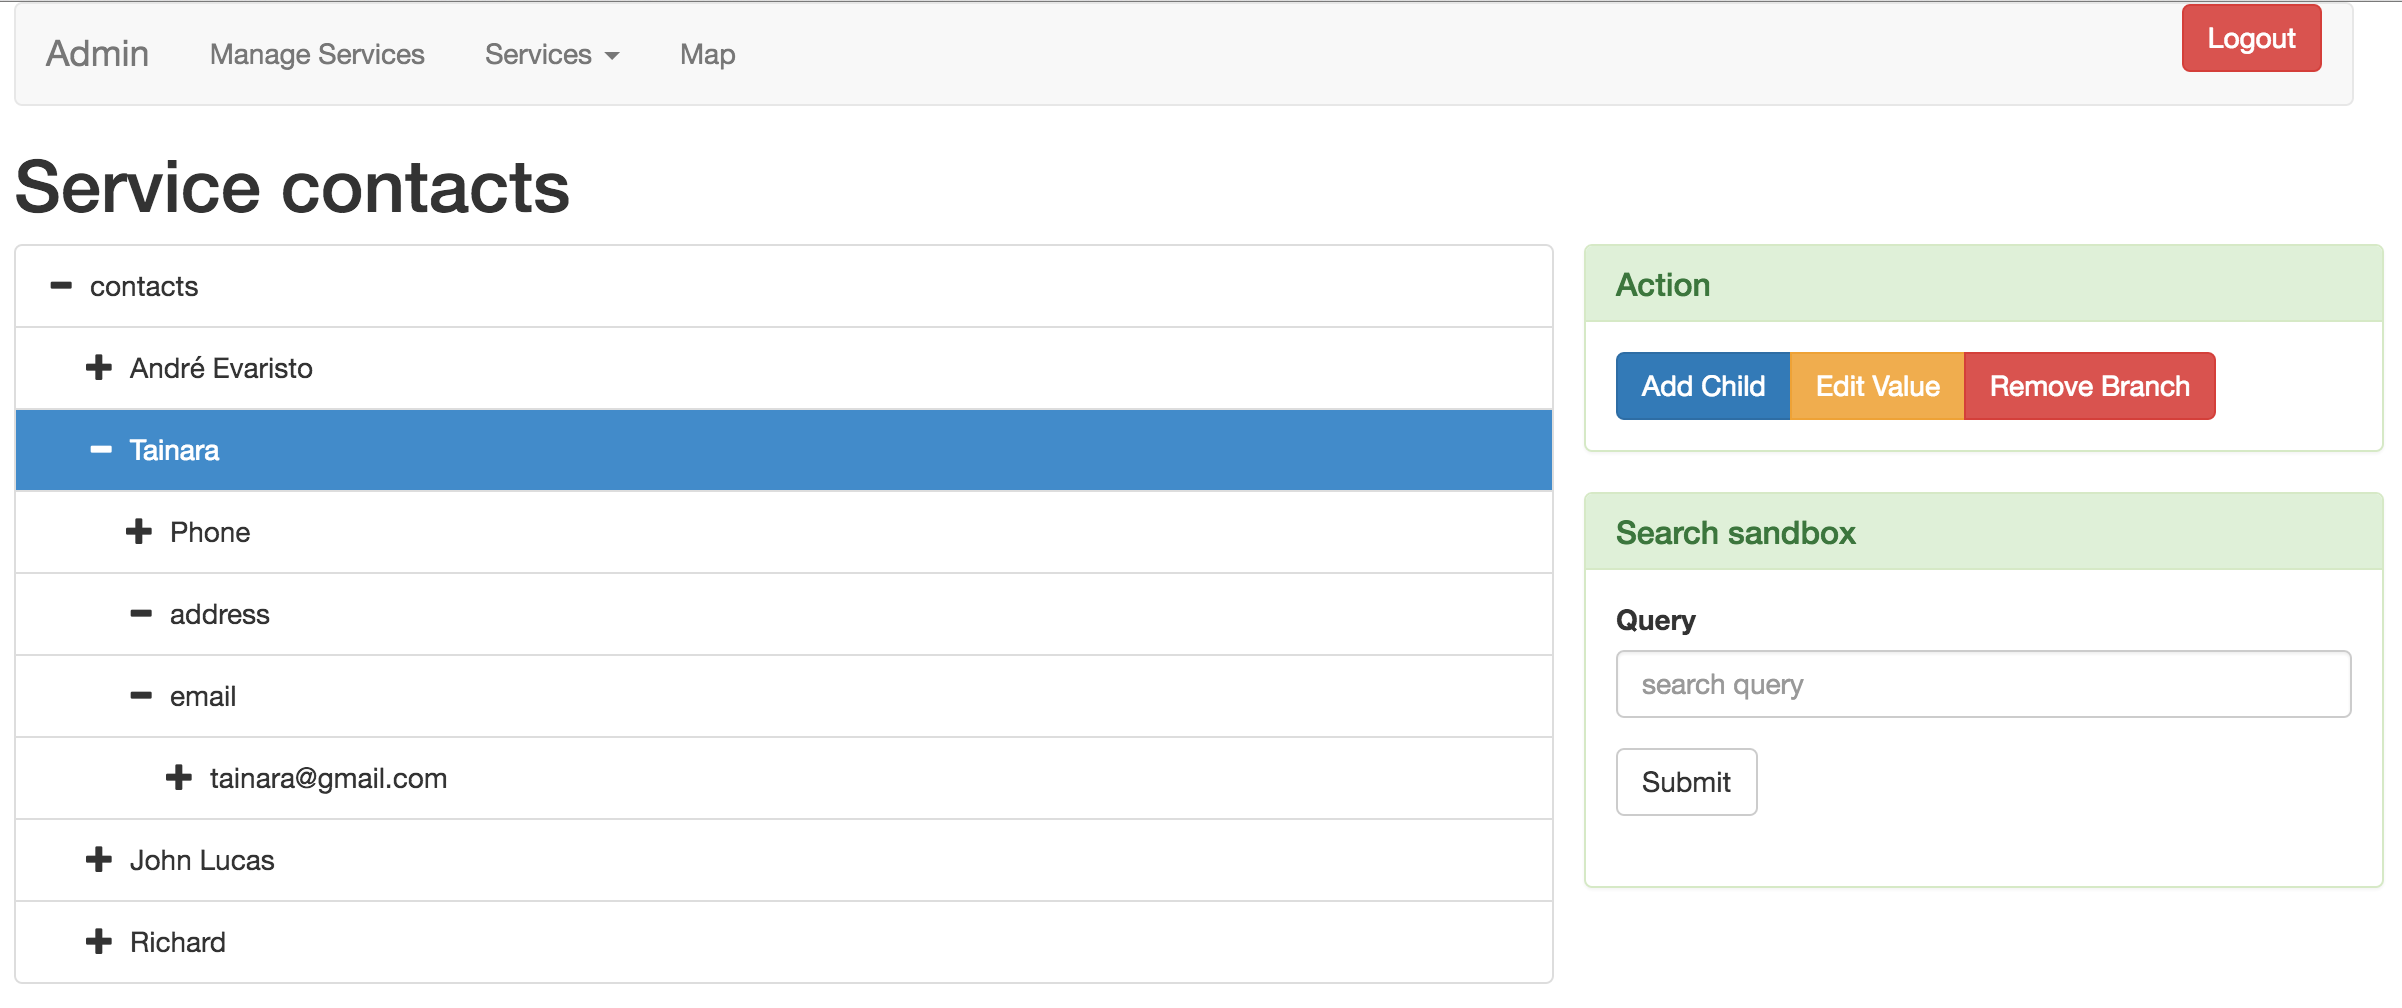
\includegraphics[width=\textwidth]{figures/services.png}
\caption{Editing a data service within the administrator screen: the knowledge tree can be fully edited visually and a search query can be tested on the fly.}
\label{fig:sys_serv}
\end{center}
\end{figure}

Lastly, a setting page for the indoor navigation was also created.
As aforementioned, this feature is not available in this version of the system due to technical problems faced during the implementation.
(For more details, see Section \ref{sec:ex-project}).
Anyway, the configuration page allows the administrator to set sizes of the map presented to the user, as well as the accuracy used when answering localization queries.

\begin{figure}[htbp]
\begin{center}
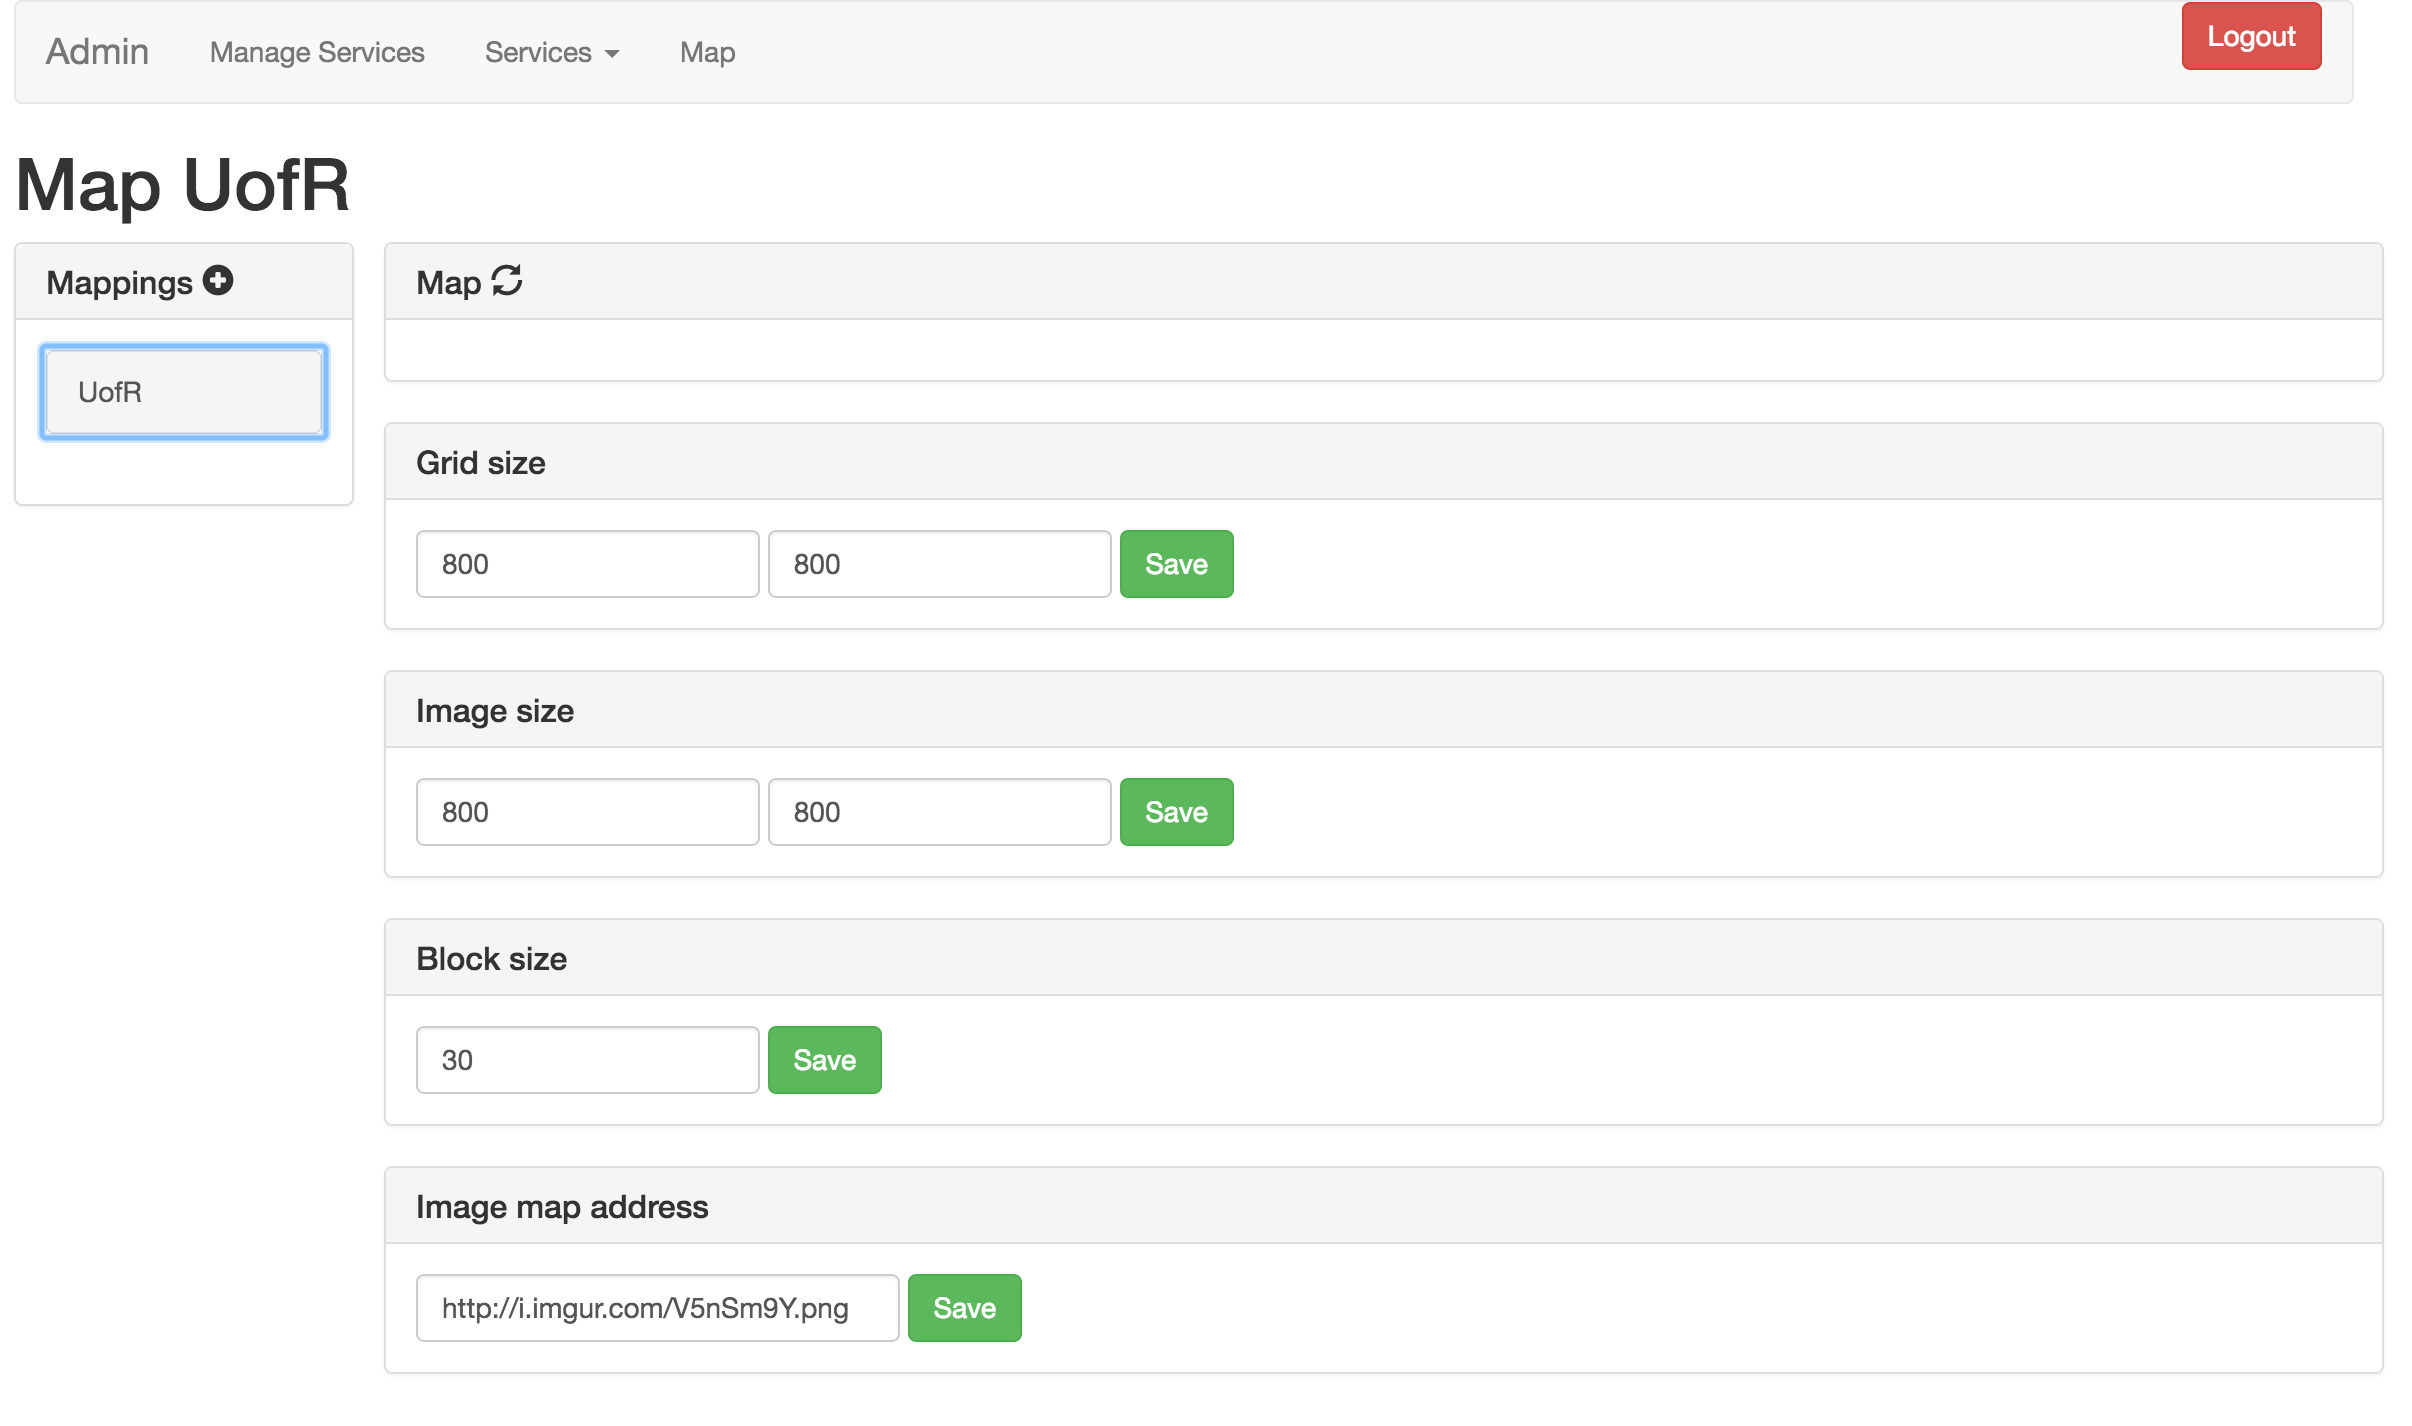
\includegraphics[width=\textwidth]{figures/map.png}
\caption{Future works include indoor navigation capabilities allowing the administrator to set up this service from within the administration screen.}
\label{fig:sys_serv}
\end{center}
\end{figure}
